% !TeX encoding = UTF-8
\documentclass[a4paper,12pt]{article}
\usepackage{ctex,geometry,graphicx,tikz,setspace,paralist,fancyhdr,caption,ulem,amsmath,verbatim}
\geometry{
	left=2cm,
	right=2cm,
	top=2cm,
	bottom=2cm,}
\renewcommand{\maketitle}{
	\begin{titlepage}
		\begin{center}
			
\includegraphics[width=0.4\textwidth]{1_1.png} % 插入你的公司/机构logo
			\vspace{4cm}
			
			\zihao{1} \textbf{数值计算\\期中大作业} \\
			\vspace{2cm}
			
			\zihao{3} 专业:\uline{通信工程} \\
			\vspace{0.5cm} 
			\zihao{3} 学号:\uline{22309080} \\
			\vspace{0.5cm} 
			\zihao{3} 姓名:\uline{梁倍铭} \\
			\vspace{0.5cm} 
			\zihao{3} 时间:\uline{2023.1.18} \\
			\vfill
		\end{center}
	\end{titlepage}
}
\begin{document}
	\maketitle
	\tableofcontents
	\newpage
	\large
	\onehalfspacing
	\section{前言}
	在期中报告中已完成了对《[1] Efficient Algorithm for Detecting Layered Space Time Codes》和《[2] MMSE Extension of V-BLAST based on Sorted QR Decomposition》这两篇论文中V-BLAST、QRD、SQRD、ZF、MMSE、MMSE-QRD和MMSE-SQRD算法的仿真复现。\par 
	在期末报告中,将完成对MMSE-QRD-PSA、基于信道矩阵SVD分解的发送与检测、基于信道矩阵GMD分解的发送与检测的仿真实现,并通过计算误码率和误帧率来比较他们的性能差异。
	\section{系统模型}
	系统模型为MIMO系统,在期中报告中已经给出。\par 
	MIMO全称是multiple-in multiple-out,多输入多输出。示意图如图1,具有$N_T$根发射天线和$N_R$根接收天线,且$N_R>N_T$,数据在$N_T$个等长的数据子流(称为层)中进行解复用。这些子流被映射成M-PSK或M-QAM符号,或者,可以使用前向纠错(FEC)码在映射之前对数据子流进行编码。\par 
	\begin{figure}[h]
		\centering
		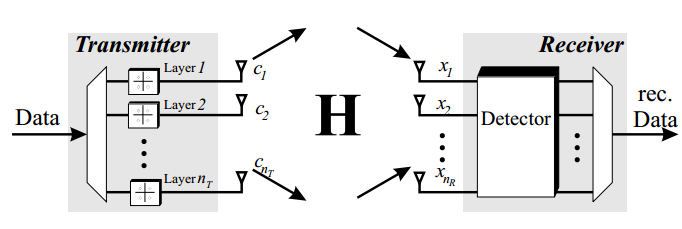
\includegraphics[width=0.5\textwidth]{1.png}
		\caption{MIMO系统示意图}
	\end{figure}
	用$c=\begin{pmatrix}
		c_1&c_2&\dots &c_{nt}
	\end{pmatrix}^\top $来表示发射的信号,用$x=\begin{pmatrix}
		x_1&x_2& \dots &x_{nr}
	\end{pmatrix}$来表示接收到的信号。信道H的大小为$N_T*N_R$,信道H可表示为$$H=\begin{pmatrix}
		h_{1,1}& \dots & h_{1,nT} \\
		\cdots &	\cdots	& \cdots \\
		h_{nR,1}& \dots & h_{nR,nT}
	\end{pmatrix}$$
	由于两篇论文所使用的符号不尽相同,这里采用第一篇论文的符号进行统一描述,用v来表示接收天线中的高斯白噪声,
	$v=\begin{pmatrix}
		v_1&v_2& \dots & v_{NR}
	\end{pmatrix}^\top$,因此,整个系统可以用$x=Hc+v$来描述。\par 
	其中我们假设假设所有天线每维的方差 N0=2 的不相关高斯白噪声。传输的符号被归一化,使得每比特的平均接收能量为一。我们假设静态平坦衰落环境,即信道矩阵 H 在帧内保持不变,并且在帧与帧之间独立变化。假定不同的衰落增益是不相关的并且接收机完全了解这些增益。
	\section{算法实现}
	\subsection{MMSE-SQRD算法的仿真实现}
	MMSE算法通过最小化实际传输符号与线性检测器输出之间的均方误差 (MSE),并得出滤波器矩阵:	$$G_{MMSE}=(H^HH+\sigma^2I_{nT})^{-1}H^H$$
	进而得到检测信号:
	$$\hat{c}_{MMSE}=H^{+}x$$
	结合QR算法,为了获得最优的检测顺序,可以通过在每个正交化步骤之前对信道矩阵的列进行重新排序,来提高检测性能。伪代码如图2.\par 
	\begin{figure}[h]
		\centering
		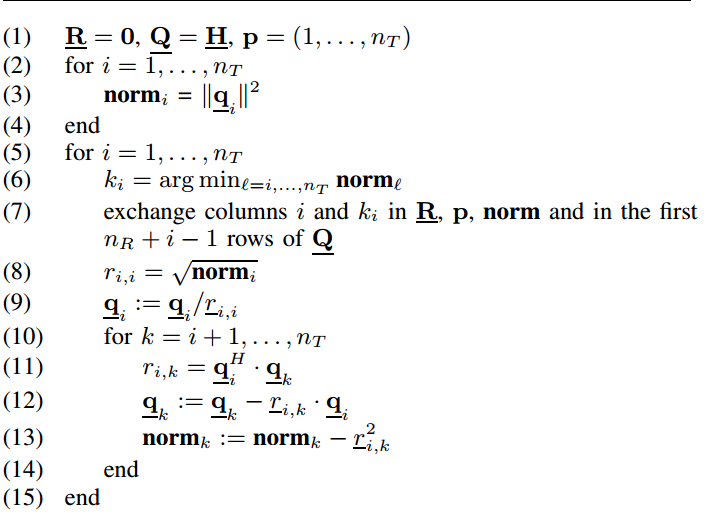
\includegraphics[width=0.7\textwidth]{2.png}
		\caption{MMSE-SQRD伪代码}
	\end{figure}
	matlab代码如图3.
	\newpage
	\begin{figure}[h]
		\centering
		\begin{minipage}{0.45\textwidth}
			\centering
			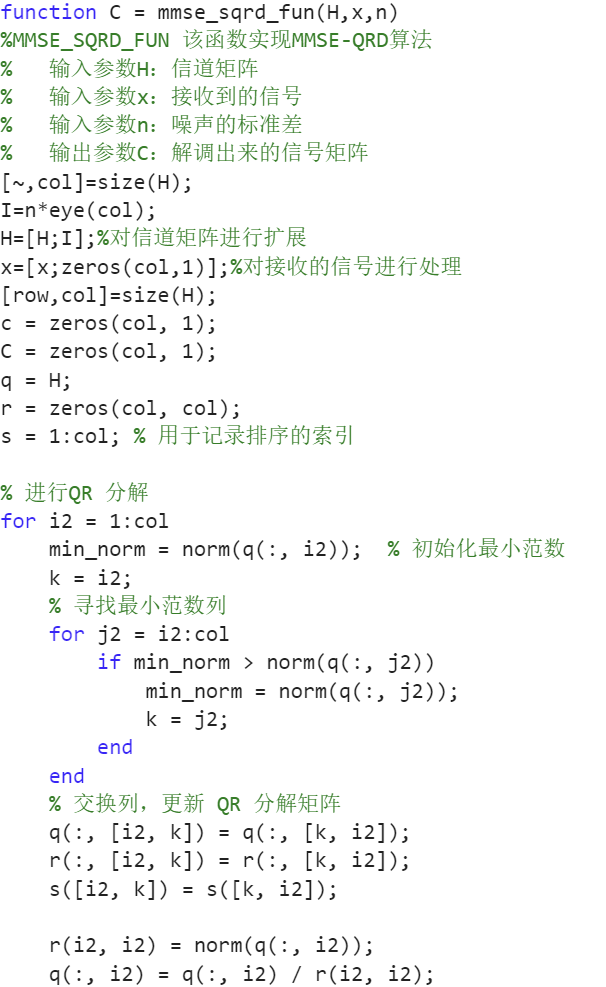
\includegraphics[width=\textwidth]{3.png}
		\end{minipage}
		\qquad
		\begin{minipage}{0.45\textwidth}
			\centering
			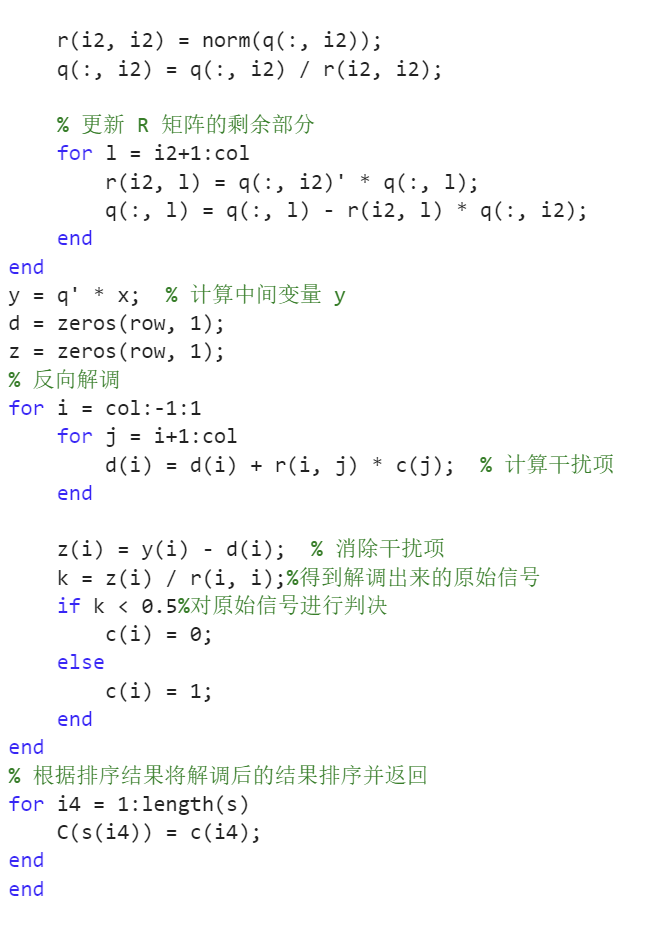
\includegraphics[width=\textwidth]{4.png}
		\end{minipage}
		\caption{MMSE-SQRD伪代码}
	\end{figure}
	\subsection{MMSE-SQRD-PSA算法的仿真实现}
	由于协方差误差矩阵$\Phi$可以写成$\Phi=Q_2Q_2^H$,由于$Q_2$是上三角的,$\Phi$的第k个对角元素与$Q_2$第k行的范数成正比,在最优排序算法中,$Q_2$的最后一行必须具有所有行的最小范数。\par 
	若满足该条件,则$Q_2$左上$n_T-1\times n_T-1$子矩阵的最后一行必须具有该子矩阵所有行的最小范数,如果排序正确,则此条件由所有左上子矩阵完成。\par 
	若矩阵$Q_2$不满足该条件。那么范数最小的行和最后一行需要交换,通过将$Q_2$的置换版本与适当的酉$n_T\times n_T$Householder反射矩阵$(\Phi)$相乘得到分块三角矩阵。最后,$Q_1$更新为$Q_1\Phi$,在PSA结束时反转$Q_2$。\par 
	然后针对修改后的矩阵$Q_2$的左上$n_T-1\times n_T-1$子矩阵和新矩阵$Q_1$的前$n_T-1$列迭代这些排序和反射步骤,从而产生 QR 分解最优排序的信道矩阵 H.\par 
	伪代码如图4,在MMSE-SQRD的基础上增加的matlab代码如图5
	\newpage
	\begin{figure}[h]
		\centering
		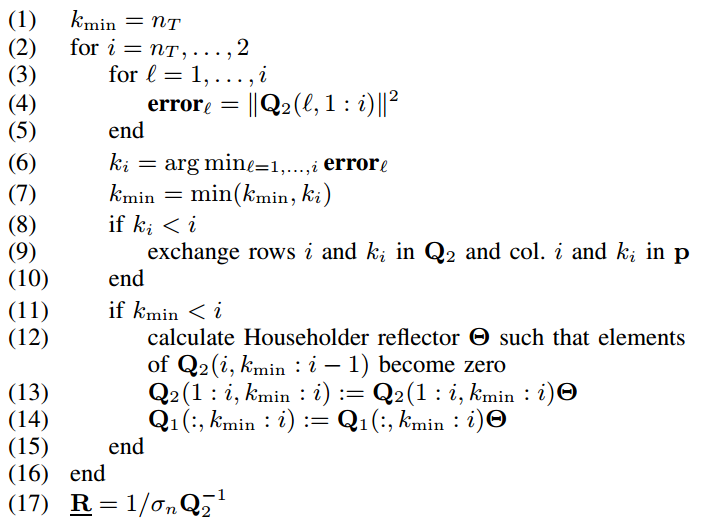
\includegraphics[width=0.5\textwidth]{5.png}
		\caption{MMSE-SQRD-PSA伪代码}
	\end{figure}
	\begin{figure}[h]
		\centering
		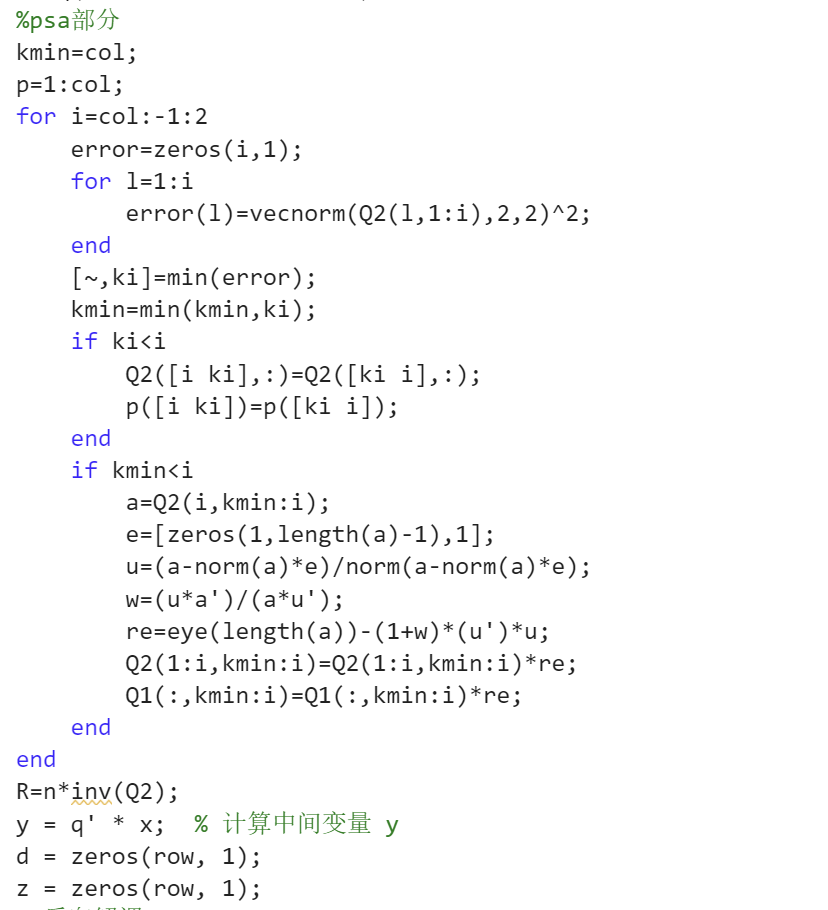
\includegraphics[width=0.5\textwidth]{6.png}
		\caption{MMSE-SQRD-PSAmatlab代码}
	\end{figure}
	\subsection{基于信道矩阵SVD分解的发送与检测的仿真实现}
	奇异值分解(Singular Value Decomposition,以下简称SVD)是一种广泛使用的算法,SVD并不要求要分解的矩阵为方阵,他将矩阵(A)分解为正交矩阵(U),对角矩阵($\Sigma$)和正交矩阵(V)。即$A=U\Sigma V$.\par 
	在MIMO系统中,可以对信道矩阵进行SVD分解
	$$H=U\Sigma V$$
	系统函数变成$$x=U\Sigma Vc-v$$
	令$$y=U'x$$
	$$s=Vc$$
	则$$y=\Sigma s+U'v$$
	所以在接收端和发射端分别乘一个矩阵,目的是为了得到一个干净的传输矩阵,也就是对角线矩阵。\par 
	在进行仿真时,我们只需对前面的代码稍作修改,便可实现基于信道矩阵SVD分解的发送与检测。假设将信号矩阵H分解成$U\Sigma V$,即$H=U\Sigma V$,在发送c时,左乘V,如图6,在接收端,信道矩阵H变成了$\Sigma$,将接收到的x左乘U的逆,如图7
	\begin{figure}[h]
		\centering
		\begin{minipage}{0.45\textwidth}
			\centering
			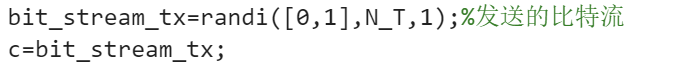
\includegraphics[width=\textwidth]{7.png}
		\end{minipage}
		\qquad
		\begin{minipage}{0.45\textwidth}
			\centering
			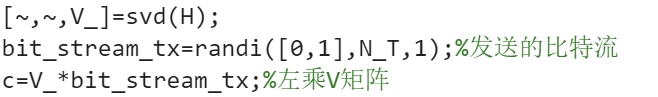
\includegraphics[width=\textwidth]{8.png}
		\end{minipage}
		\caption{SVD发射端对比matlab代码}
	\end{figure}
	\begin{figure}[h]
		\centering
		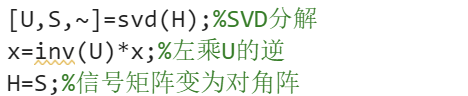
\includegraphics[width=0.5\textwidth]{9.png}
		\caption{SVD接收端增加的matlab代码}
	\end{figure}
	\subsection{基于信道矩阵GMD分解的发送与检测}
	GMD(几何均值分解)的思想和SVD类似,都是在接收和发射端同时对信号进行处理。处理过程如下:\par
	将信道矩阵进行GMD分解:
	$$H=QRP'$$
	对发送信号进行处理:
	$$x=Ps$$
	系统模型变为:
	$$y=QRs+z$$
	对其进行解调即可得到发射信号s,发射端代码如图8,接收端代码如图9.
	\begin{figure}[h]
		\centering
		\begin{minipage}{0.45\textwidth}
			\centering
			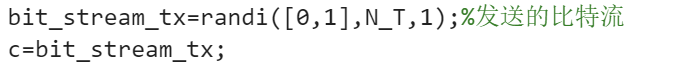
\includegraphics[width=\textwidth]{7.png}
		\end{minipage}
		\qquad
		\begin{minipage}{0.45\textwidth}
			\centering
			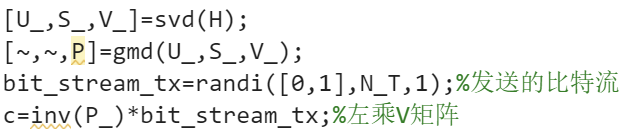
\includegraphics[width=\textwidth]{10.png}
		\end{minipage}
		\caption{GMD发射端对比matlab代码}
	\end{figure}
	\begin{figure}[h]
		\centering
		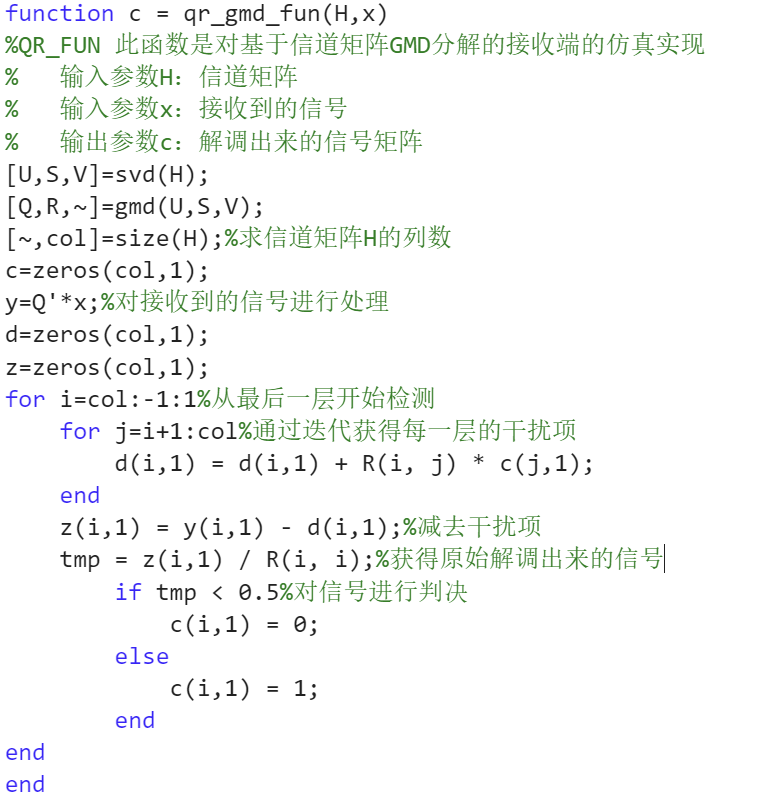
\includegraphics[width=0.5\textwidth]{11.png}
		\caption{GMD接收端的matlab代码}
	\end{figure}
	\section{对各项算法的测试}
	\subsection{MMSE-SQRD和MMSE-SQRD-PSA与期中各个算法对比}
	假设接收天线为8,发射天线为6,测试100000次,并统计各个算法的无码率,测试结果如图10.\par 
	\begin{figure}[h]
		\centering
		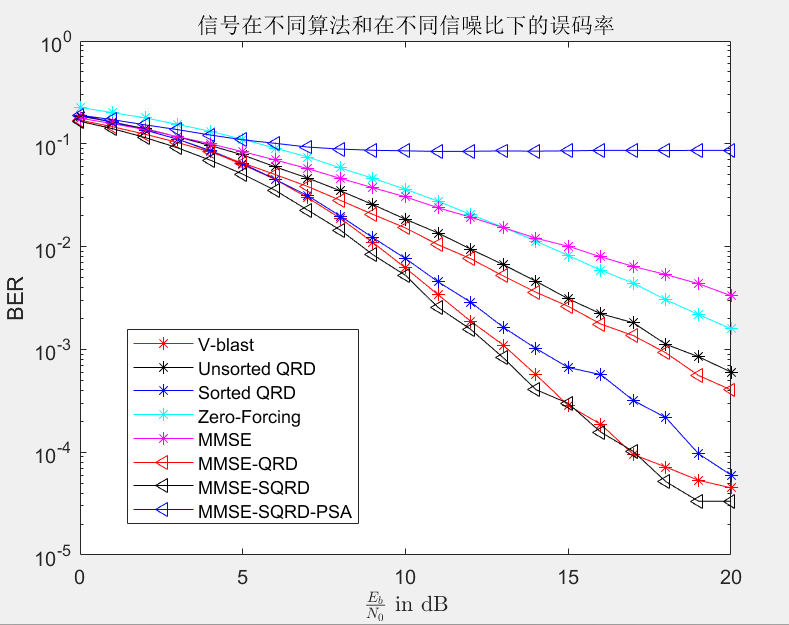
\includegraphics[width=0.5\textwidth]{12.png}
		\caption{测试结果1}
	\end{figure}
	假设接收天线为12,发射天线为8,测试100000次,并统计各个算法的误码率,测试结果如图11.\par 
	\begin{figure}[h]
		\centering
		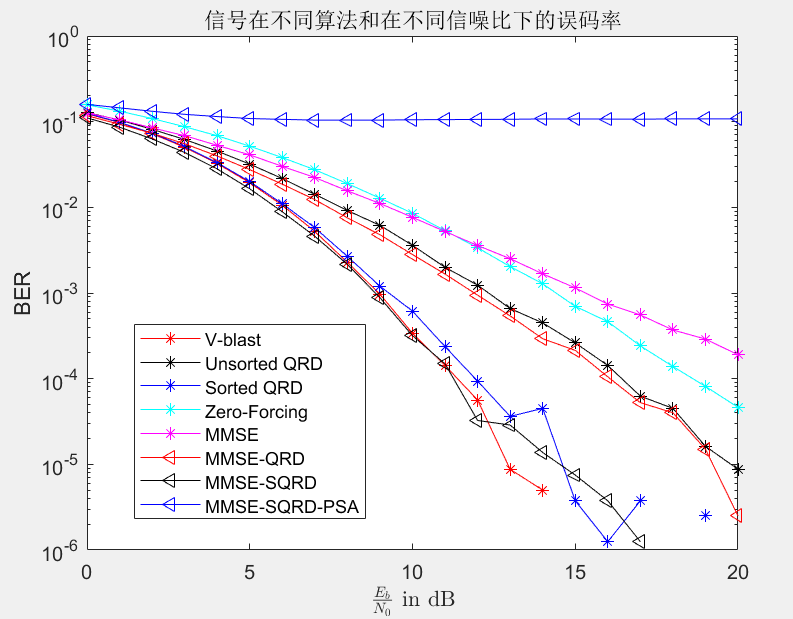
\includegraphics[width=0.5\textwidth]{13.png}
		\caption{测试结果2}
	\end{figure}
	\newpage
	从测试结果可以看出,MMSE-SQRD算法和V-BLAST算法的误码率最低,然后到SQRD算法,紧接着是MMSE-QRD和QRD算法,最后是MMSE和ZF算法,结合算法复杂度,不考虑MMSE-SQRD-PSA的情况下,MMSE-SQRD的综合性能最好。图中观察可知MMSE-SQRD-PSA的算法误码率明显偏高,单独测试MMSE-SQRD-PSA算法,测试结果如图12.\par 
	\newpage
	\begin{figure}[h]
		\centering
		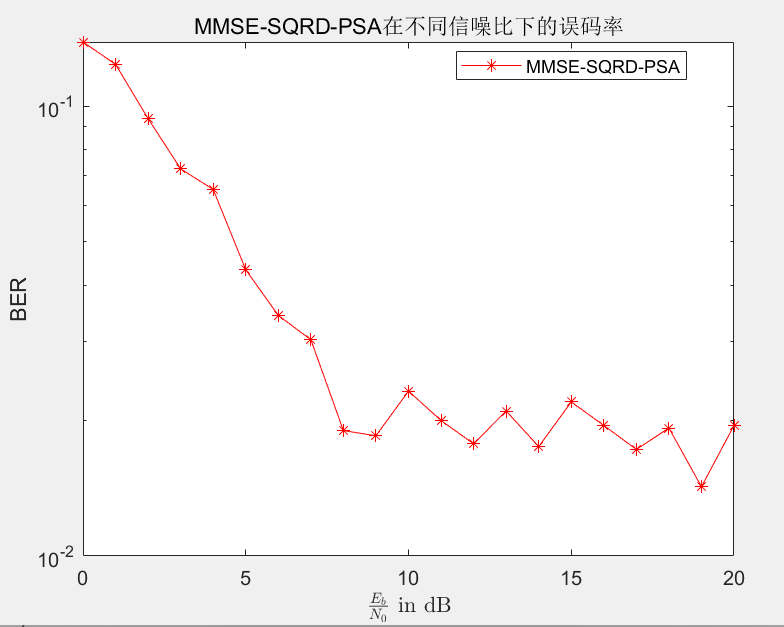
\includegraphics[width=0.5\textwidth]{14.png}
		\caption{测试结果3}
	\end{figure}
	从测试结果来看,MMSE-SQRD-PSA算法误码率在0.01和0.1之间,说明还是存在问题,但是debug了好久,仍然没有发现出错的地方,因此此处没有完全完成。
	\subsection{SVD、GMD与其他算法对比}
	\subsubsection{对比SVD对V-blast和ZF算法的影响}
	假设接收天线为8,发射天线为6,测试100000次,并统计各个算法的无码率,测试结果如图13.\par 
	\begin{figure}[h]
		\centering
		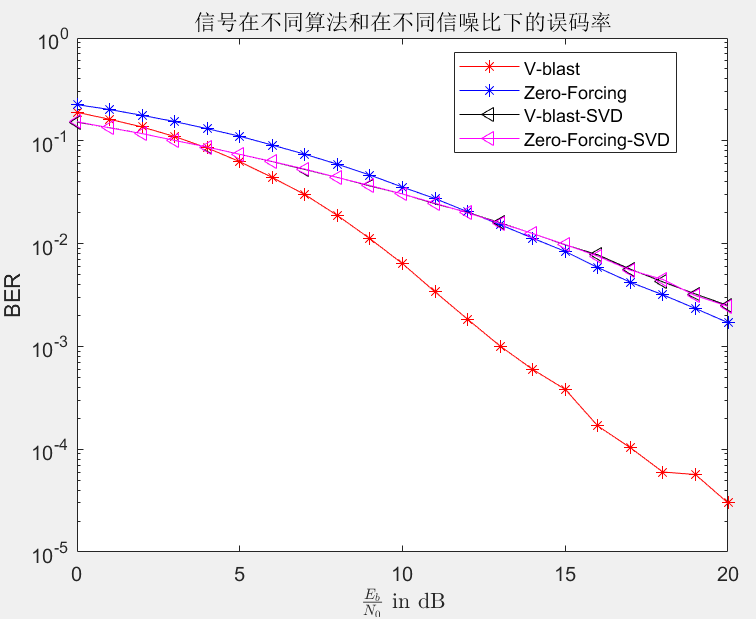
\includegraphics[width=0.5\textwidth]{15.png}
		\caption{测试结果4}
	\end{figure}
	从图中可以看出,进行SVD分解后,可能会导致误码率偏高,但是由于信号矩阵变为了对角阵,大大简化了运算
	\subsubsection{对比GMD对QRD算法的影响}
	假设接收天线为8,发射天线为6,测试1000000次,并统计各个算法的无码率,测试结果如图14.\par 
	\begin{figure}[h]
		\centering
		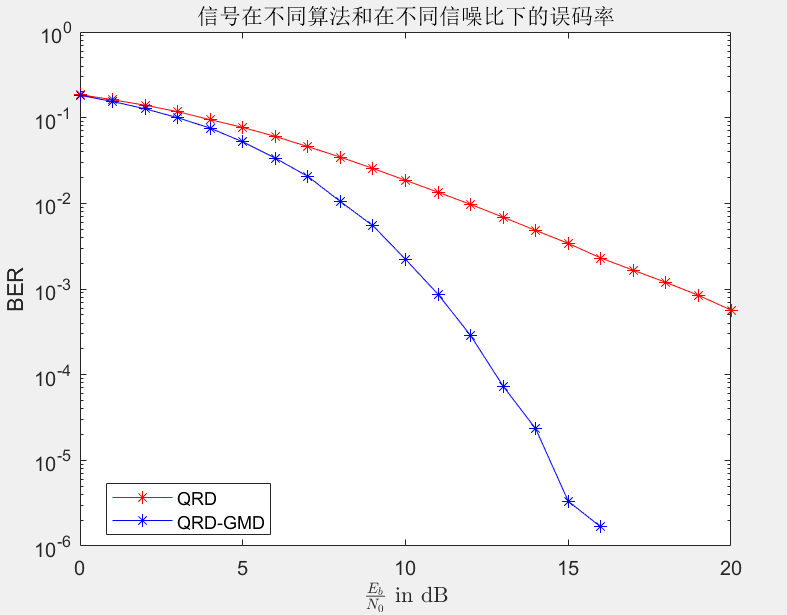
\includegraphics[width=0.5\textwidth]{16.png}
		\caption{测试结果5}
	\end{figure}
	从图中可以看出,进行GMD分解后,大大降低了QR分解的误码率,提高了系统性能。
	\section{源代码附件说明}
	\subsection{测试说明}
	直接运行main.m文件即可,为了测试方便,已经将测试次数改小。
	\subsection{源码说明}
	\begin{enumerate}
		\item bertest*文件,用来生成随机H和x矩阵。
		\item compare*文件,用来调用测试文件和算法文件来进行测试并绘图
		\item 以算法命名的文件,每个文件代表一个算法。
		\item  main.m文件,主测试文件,直接运行即可测试。
	\end{enumerate}
\end{document}